\chapter{Design and Implementation} %(approx. 10 pages)\\

\section{Program Design and Interaction Mechanisms} %TODO: Everybody, yeaahhhh ;)
* Approach to design\\
* important issues and choices and their relationships to theoretical concepts and the hardware and software platforms\\
* Did you use the GPIO module? How? In terms of interrupts and the setup in the main\\
* Did you use interrupts? How?\\ 
* Did you use multiple threads / handlers? How? Why?\\
* Did you use TI-RTOS? How?\\

\section{State Machine} %TODO: Hendrik
To control the program flow, state machines are a suitable approach for real-time software (Lecture 2). They allow design for multi-threaded software and real-time events can be used to cause state changes. By implementing the state machine in one task, concurrency with other parts of the software is no problem because the state machine task can sleep between iterations and change its state based on events or the result values of methods called from inside the states. Even though they can not depict time constraints in every case. Tasks which are time critical should not be implemented or called inside a specific state to ensure real-time responses.

The state machine (see Fig.\ref{fig:statemachine}) is executed in an own task inside an infinite while loop with a sleep of 10 ticks between each iteration. The execution starts in the \texttt{INIT} state. There the related method from the driver library is called to set up and initialize data structures. If the method return true as an indication that it was successful, the current state is changed to \texttt{INIT\_STATION}. Again the related function from the driver library is called, this time to ensure that the platform is in its initial position and the ejector is retracted. The functions in the driver library are all implemented as blocking functions with a return value to indicate their success in execution. After successfully returning from the method call, the state will be changed to the \texttt{CHECK\_WORKPIECE} state. In this state it will only be checked if a work piece was placed in the designated position on the platform. The switching to the next state will only be executed, if the return value indicated an available work piece.
To ensure a safe testing process the moving parts will not be activated before the state \texttt{CHECK\_SAFTEY\_BARRIER} was executed and indicated a clear working zone. The state is then changed to \texttt{MEASURE\_WORKPIECE}. This state is the most important and complex one. With the platform still remaining in the bottom position, the material and color is retrieved through a driver library function call and saved into a struct which is defined in the libraries header file. Then the platform is moved up to get the height measurement from the sensor at the top. The movement of the platform is stopped by an hardware interrupt outside of the state machine. The corresponding method will return true when the top position is reached and after a little delay a measurement is triggered. This is also saved into global variable and afterwards the method \texttt{checkWorkpiece()} is called to decide if the work piece is accepted or rejected. This decision can be made based on the data available in the struct and the height variable, but in the current implementation only the height of the work piece is relevant and the material and colour are only logged for statistic purposes. The state should change to \texttt{ACCEPT\_WORKPIECE} or \texttt{REJECT\_WORKPIECE} afterwards. In case something goes wrong when moving the platform up (which would be indicated by the return value of the \texttt{movePlattform()} method), the state is changed back to \texttt{INIT\_STATION} and the checks and measurement will be repeated.
The \texttt{ACCEPT\_WORKPIECE} state first activates the air slider and then triggers a cascade of method calls to extend the ejector, retract the ejector, move the platform down and switch the air slider off again. If one of the first three methods fail the current state is changed to \texttt{INIT\_STATION} and the air slider is turned off, otherwise the new state will be \texttt{CHECK\_WORKPIECE}. Then the next work piece can be inserted and the testing process will continue.
If the work piece is rejected after the measurements, inside the \texttt{REJECT\_WORKPIECE} state as well a cascade of method calls is executed, to move the platform down, extend the ejector and retract the ejector. In any error case we return to our initialisation state of the station or in case of success the we continue in the \texttt{CHECK\_WORKPIECE} state.

A special case is the \texttt{CALIBRATE\_SENSOR} state. After each iteration of the state machine, it is checked whether the event with the ID 04 has occurred. If this is the case, the current state is changed to start the calibration, no matter if it was changed before or would just stay the same. The event is triggered by a click on the hardware up  button next to the display. Inside the state the method to execute the calibration procedure is called, then the movement of the platform is disabled to allow the operator to remove the calibration work piece manually. After that the state machine changes to the \texttt{INIT\_STATION} state.

\begin{figure}[H]
	\begin{center}
		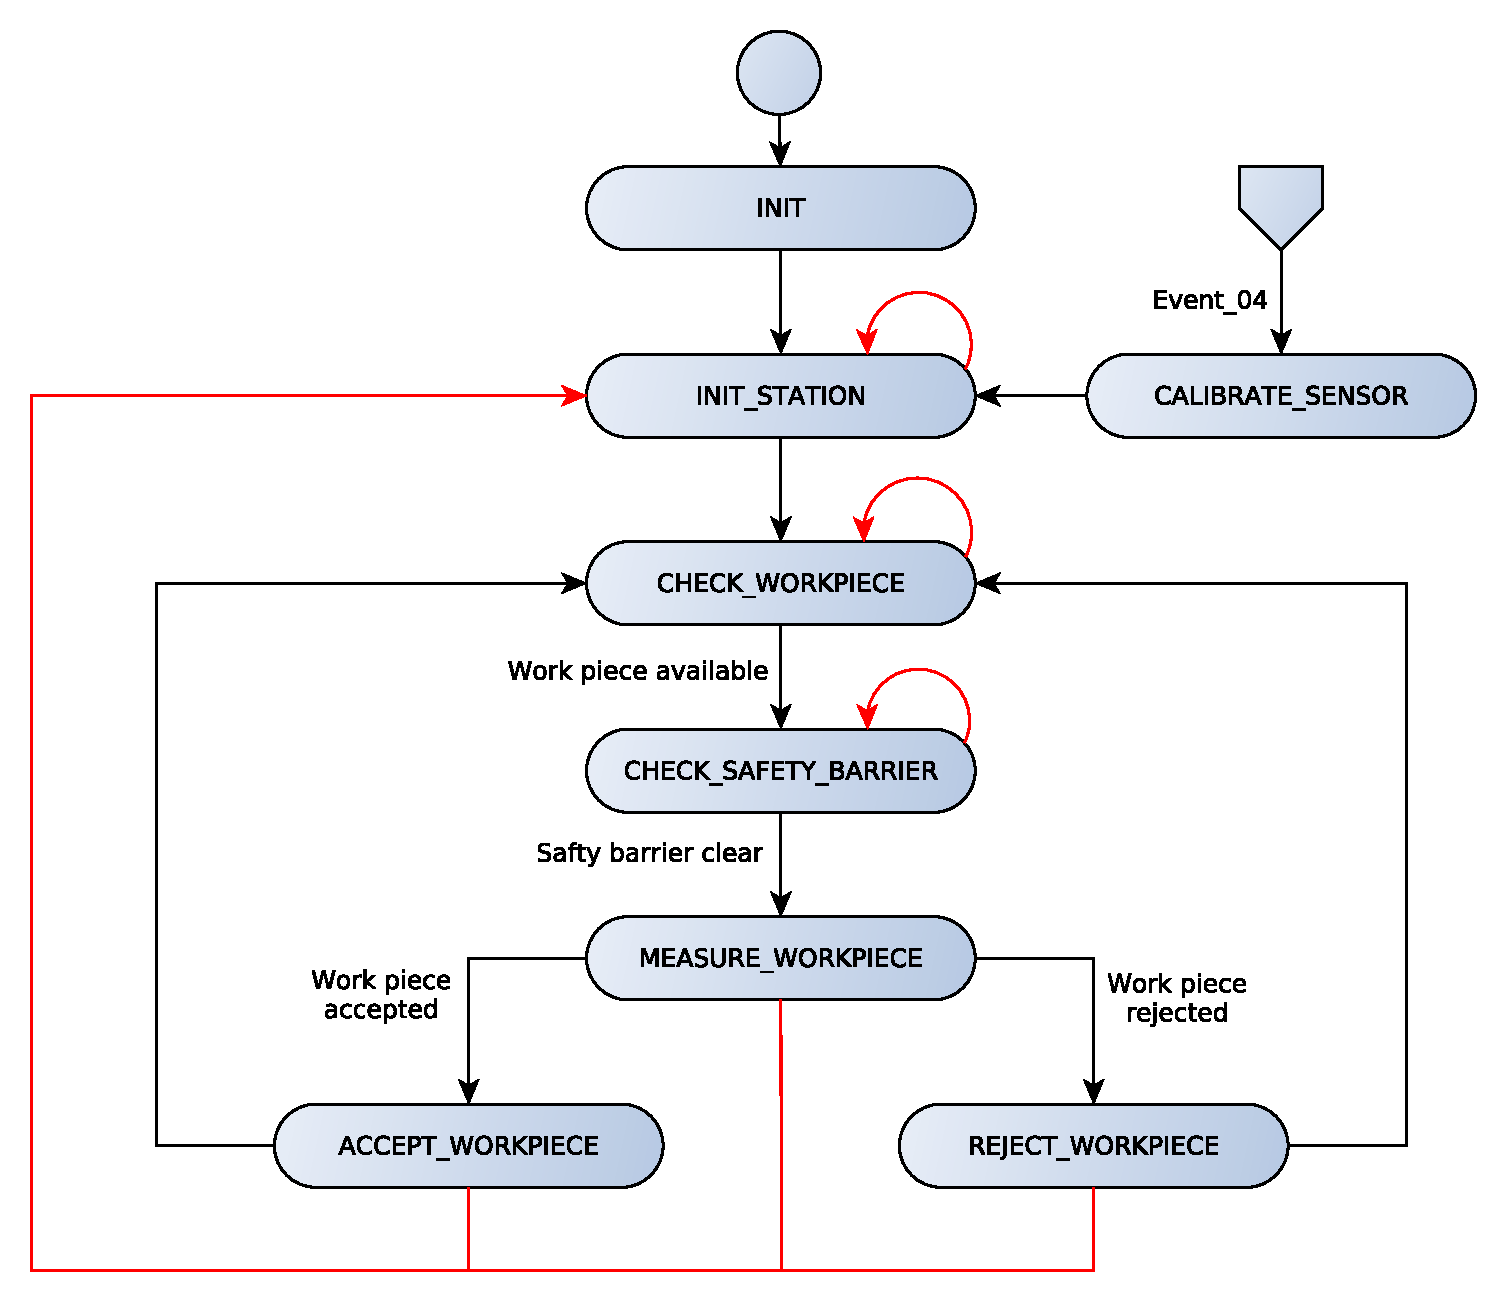
\includegraphics[scale=.60]{media/StateMachine_Main.pdf} 	
		\caption{Main State Machine}
		\label{fig:statemachine}
	\end{center}
\end{figure}

\section{Calibration} %TODO: Hendrik

\section{Device Driver Library} %TODO: Timo
* Did you use the GPIO module? How? Through the qut library... Pin Map table?\\
* Did you use the ADC? How? 

% TODO: Table of measurements?

\begin{figure}[H]
	\begin{center}
		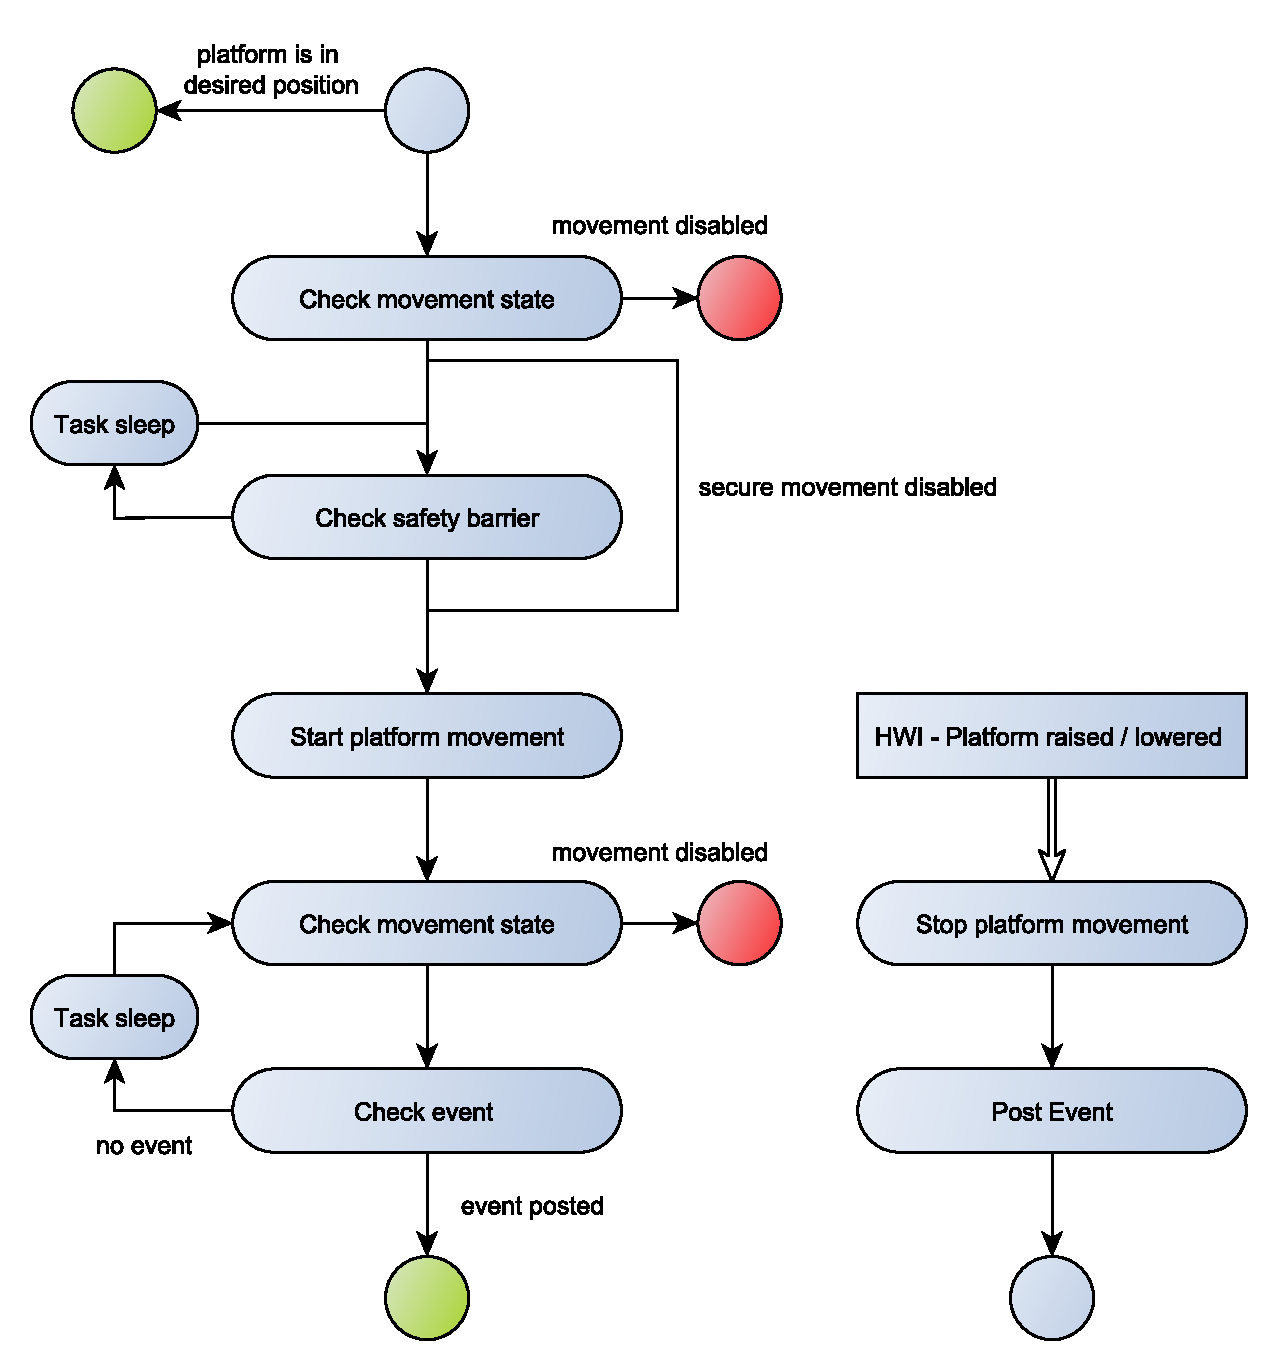
\includegraphics[scale=.60]{media/Flow_Chart_MovePlatform.pdf} 	
		\caption{Flow Chart Move Platform}
		\label{fig:moveplatform}
	\end{center}
\end{figure}

\section{User Interface} %TODO: Pixel-Julian
* Did you use the graphics library? How?\\



